\documentclass[a4paper,12pt]{article}

% ==============================
%            ПАКЕТЫ
% ==============================
\usepackage{cmap}
\usepackage[T2A]{fontenc}
\usepackage[utf8]{inputenc}
\usepackage[english,russian]{babel}
\usepackage{hyperref}
\usepackage{multicol}
\usepackage{mathtools}
\usepackage{amssymb}
\usepackage{enumitem}
\usepackage{tikz}
\usepackage{cancel}
\usetikzlibrary{automata, positioning, arrows.meta}
\usepackage[linesnumbered,ruled,vlined]{algorithm2e}


% ==============================
%         СОКРАЩЕНИЯ
% ==============================
\newcommand{\T}{\mathcal{T}}
\newcommand{\w}{\omega}
\newcommand{\pair}[2]{\langle #1, #2 \rangle}

% ==============================
%         ТИТУЛЬНЫЙ ЛИСТ
% ==============================
\begin{document}

\begin{titlepage}
\centering

{\LARGE \textbf{Теория формальных языков} \par}
\vspace{0.5cm}

{\large \textbf{Лабораторная работа №2} \par}
{\large Вариант 8 \par}
\vspace{1.5cm}

{\large \textbf{Работу выполнила:} \par}
{\large Студент группы ИУ9-51Б \par}
{\large Григорьева Софья \par}

\end{titlepage}


% ==============================
%         СОДЕРЖАНИЕ
% ==============================

\tableofcontents
\newpage

% ==============================
%           ЗАДАНИЕ
% ==============================

\section{Задание}

Дано регулярное выражение:
\[
((aa | ba)(ab)^*(bb)^*)^*
\]

По имеющемуся академическому регулярному выражению построить:

\begin{itemize}
\item Минимальный ДКА, распознающий его язык (минимальность обосновать таблицей классов эквивалентности)
\item Возможно малый НКА, распознающий его язык. Возможно малый переключающийся (с конъюнкцией) КА, распознающий его язык. Частично обосновать таблицами множеств классов эквивалентности.
\item Расширенное регулярное выражение, распознающее тот же язык. В расширенном выражении можно использовать:
    \begin{itemize}
    \item wildcard-операцию $.$ для замены произвольного символа алфавита;
    \item положительную итерацию $\tau^+$ и опцию $\tau?$, где $\tau^+ = \tau\tau^*$, $\tau? = (\tau|\varepsilon)$;
    \item операции предпросмотра $\tau_0(?= \tau_1)\tau_2 \equiv \tau_0((\tau_1.^*) \cap \tau_2)$ и ретроспективной проверки $\tau_0(?<= \tau_1)\tau_2 \equiv (\tau_0 \cap (\tau_1.*))\tau_2$, а также их отрицательные версии $\tau_0(?! \tau_1)\tau_2 \equiv \tau_0((\tau_1.*) \cap \tau_2)$ и $\tau_0(?<! \tau_1)\tau_2 \equiv (\tau_0 \cap (\tau_1.*))\tau_2$;
    \item классы букв $[c_1 \ldots c_k] \equiv (c_1|c_2| \ldots |c_k)$ и их дополнения $[\hat{c}_1 \ldots c_k]$;
    \item (обязательно) маркеры начала и конца выражения $\hat{}$ и $\$$.
    \end{itemize}
\end{itemize}

Все конструкции выше можно делать вручную. Для их фиксации желательно использовать формат md со встроенными latex-формулами, поддерживаемыми MathJax, либо формат md обсидиана (он допускает расширенную поддержку latex в формулах). Можно и чистый latex. Допустимо сдавать и фото на листочках, но за оформление в Markdown/Latex добавляется 1 балл.

Провести автоматическое тестирование предполагаемой эквивалентности построенных распознавателей. Тем самым необходимо построить алгоритмы, определяющие принадлежность слова языку академического регулярного выражения, ДКА, НКА и ПКА.

Эквивалентность расширенного регулярного выражения тестировать не обязательно, но если сделаете распознаватель для таких выражений, то будет добавлен дополнительный балл. Если не делаете, то для расширенного регулярного выражения достаточно описать содержательно (полуформально), почему оно должно распознавать тот же самый язык.

Требуется только фазз-тестирование эквивалентности: строится случайное слово $\omega$ и проверяется, принадлежит ли он языкам регулярного выражения, ДКА, НКА и ПКА согласованно.
% -------------------------------------------------------------------------------------

\clearpage 
\section{ДКА}

\begin{figure}[!htbp]
\centering
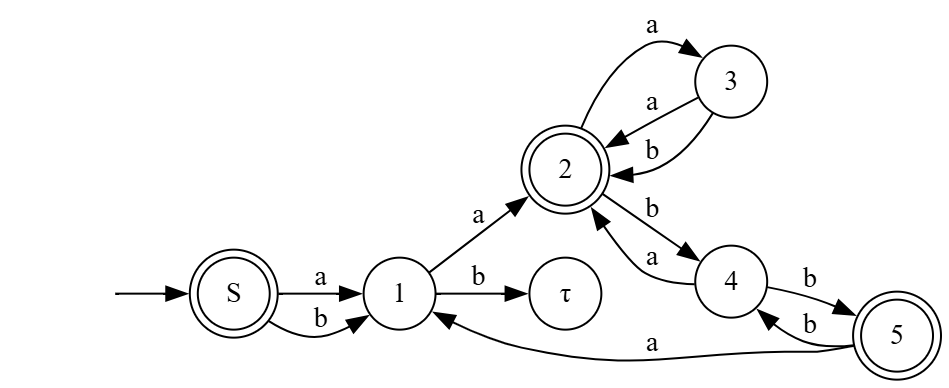
\includegraphics[width=\textwidth]{img/dka.png}
\end{figure}

\begin{table}[h!]
\centering
\begin{tabular}{|l|c|c|c|c|c|c|}
\hline
 & bb & babbb & e & b & ab \\
\hline
e & 0 & 0 & 1 & 0 & 0\\
\hline
a & 0 & 1 & 0 & 0 & 0 \\
\hline
aa & 1 & 0 & 1 & 0 & 1 \\
\hline
aaa & 0 & 1 & 0 & 1 & 0 \\
\hline
aab & 0 & 0 & 0 & 1 & 0 \\
\hline
aabb & 1 & 0 & 1 & 0 & 0 \\
\hline
ab & 0 & 0 & 0 & 0 & 0 \\
\hline
\end{tabular}
\end{table}

% digraph {
% 	rankdir = LR
% 	node [shape=circle]
% 	dummy [label = "", shape = none]
% 	0 [label="1"]
% 	1 [label="2", shape=doublecircle]
% 	2 [label="S", shape=doublecircle]
% 	dummy -> 2
% 	3 [label="3"]
% 	4 [label="4"]
% 	5 [label="5", shape=doublecircle]
% 	6 [label="τ"]
% 	0 -> 1 [label="a"]
% 	1 -> 3 [label="a"]
% 	1 -> 4 [label="b"]
% 	2 -> 0 [label="a"]
% 	2 -> 0 [label="b"]
% 	3 -> 1 [label="a"]
% 	3 -> 1 [label="b"]
% 	4 -> 1 [label="a"]
% 	4 -> 5 [label="b"]
% 	5 -> 0 [label="a"]
% 	5 -> 4 [label="b"]
% 	0 -> 6 [label="b"]
% }


\clearpage 
\section{НКА}

\begin{figure}[!htbp]
\centering
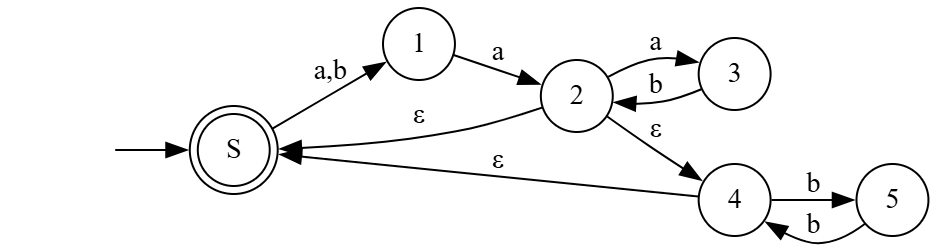
\includegraphics[width=\textwidth]{img/nka.png}
\end{figure}

\begin{table}[h!]
\centering
\begin{tabular}{|l|c|c|c|c|c|c|}
\hline
 & ab & bb & babbb & aa & b & aaa \\
\hline
aa & 1 & 1 & 0 & 1 & 0 & 0 \\
\hline
aabb & 0 & 1 & 0 & 1 & 0 & 0 \\
\hline
aaa & 0 & 0 & 1 & 0 & 1 & 1 \\
\hline
e & 0 & 0 & 0 & 1 & 0 & 0 \\
\hline
aab & 0 & 0 & 0 & 0 & 1 & 1 \\
\hline
a & 0 & 0 & 0 & 0 & 0 & 1 \\
\hline
\end{tabular}
\end{table}

% digraph {
% 	rankdir = LR
% 	node [shape=circle]
% 	dummy [label = "", shape = none]
% 	0 [label="S", shape=doublecircle]
% 	1 [label="1"]
% 	2 [label="2"]
% 	dummy -> 0
% 	3 [label="3"]
% 	4 [label="4"]
% 	5 [label="5"]
	
% 	0 -> 1 [label="a,b"]
% 	1 -> 2 [label="a"]
% 	2 -> 3 [label="a"]
% 	3 -> 2 [label="b"]
% 	2 -> 4 [label=""]
% 	4 -> 5 [label="b"] 
% 	5 -> 4 [label="b"]
% 	2 -> 0 [label=""]
% 	4 -> 0 [label=""]
% }


\clearpage 
\section{ПКА}


\begin{figure}[!htbp]
\centering
\begin{figure}
    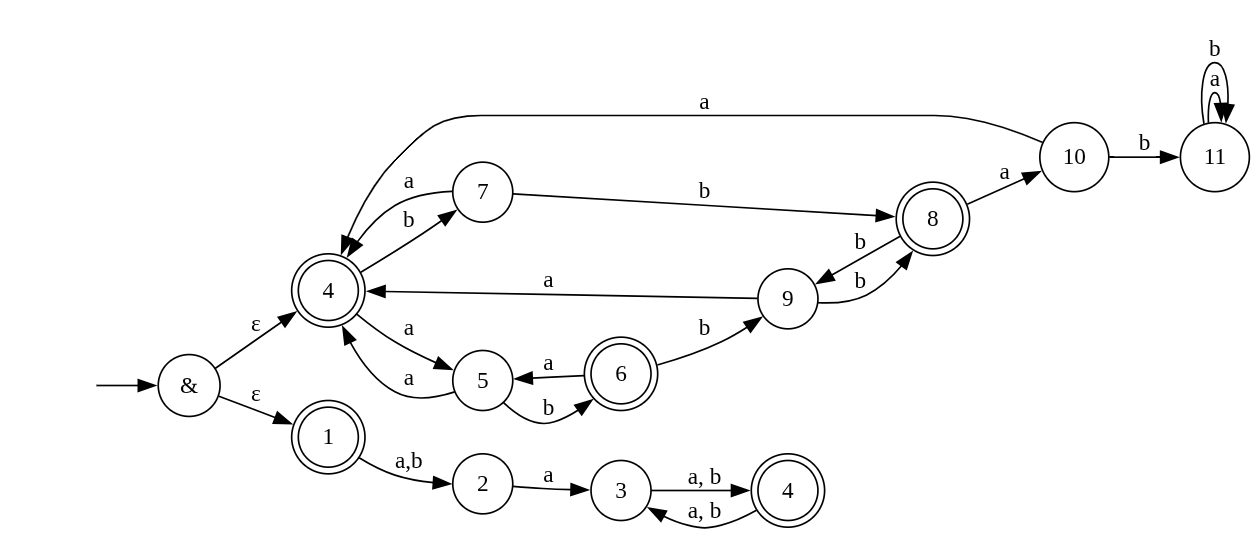
\includegraphics[width=0.5\linewidth]{img/pka.png}
    \caption{Enter Caption}
    \label{fig:placeholder}
\end{figure}
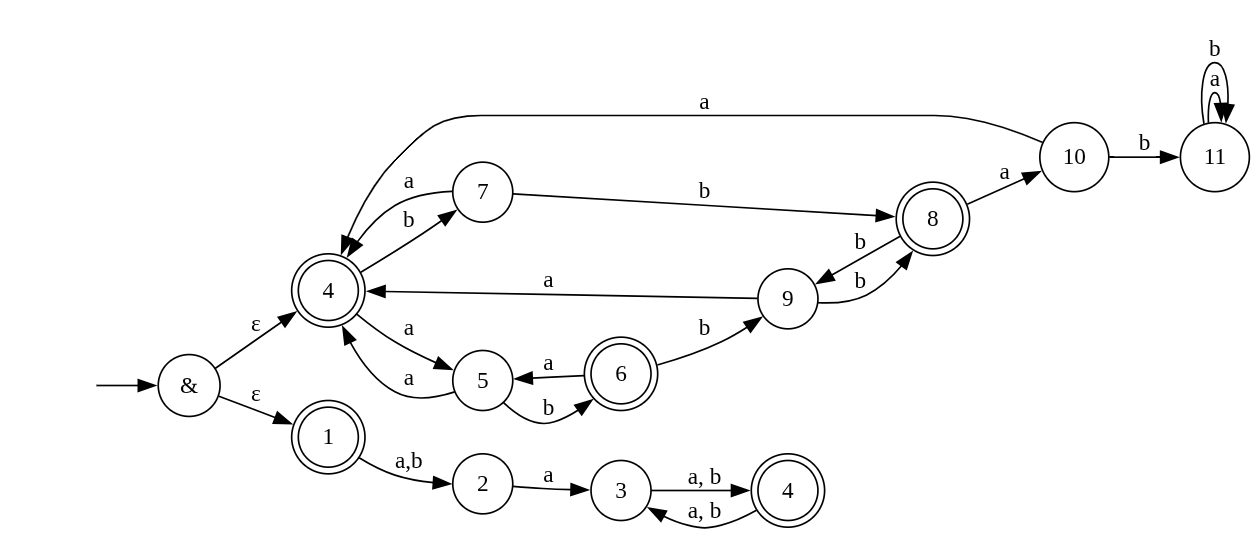
\includegraphics[width=\textwidth]{img/pka.png}
\end{figure}


\begin{table}[h!]
\centering
\begin{tabular}{|l|c|c|c|c|c|c|}
\hline
 & b & bab & aaa \\
\hline
aaa & 0 & 1 & 1 \\
\hline
b & 0 & 0 & 1 \\
\hline
bbab & 0 & 0 & 0 \\
\hline
\end{tabular}
\end{table}

% digraph DFA {
%     rankdir=LR;
%     node [shape = doublecircle]; 4 6 8;
%     node [shape = circle];
%     13 [label="&"]
%  	0 [label="1", shape=doublecircle]
%  	1 [label="2"]
%  	2 [label="3"]
%  	3 [label="4", shape=doublecircle]
%  	start [label = "", shape = none]
 	
 		
%  	start -> 13
 	
%  	13 -> 0 [label="ε"]
%  	13 -> 4 [label="ε"]
%  	0 -> 1 [label="a,b"]
%  	1 -> 2 [label="a"]
%  	2 -> 3 [label="a, b"]
%  	3 -> 2 [label="a, b"]

%     4 -> 5 [label="a"];
%     4 -> 7 [label="b"];

%     5 -> 4 [label="a"];
%     5 -> 6 [label="b"];

%     6 -> 5 [label="a"];
%     6 -> 9 [label="b"];

%     7 -> 4 [label="a"];
%     7 -> 8 [label="b"];

%     8 -> 10 [label="a"];
%     8 -> 9 [label="b"];

%     9 -> 4 [label="a"];
%     9 -> 8 [label="b"];

%     10 -> 4 [label="a"];
%     10 -> 11 [label="b"];

%     11 -> 11 [label="a"];
%     11 -> 11 [label="b"];
% }










\clearpage 
\section{Расширенное регулярное выражение}

\[
\text{\^{}}(\,.a\,(ab)^*(bb)^*)^* {\$}
\]




% -------------------------------------------------------------------------------------
\newpage
\section{Тестирование}

Исходный код программы представлен в файле <<fuzzTest.erl>>. \\ 

Программа проверяет эквивалентность трёх типов автоматов (ДКА, НКА, ПКА) и регулярного выражения через фазз-тесты на случайных словах.

В программе реализованы следующие основные функции:

\begin{itemize}[parsep=-1pt]
    \item \textbf{ДКА}:
    \begin{itemize}[parsep=-1pt]
        \item \verb|dka()| -- таблица переходов;
        \item \verb|dkaFinals()| -- финальные состояния;
        \item \verb|useDka(Word)| -- проверка слова.
    \end{itemize}

    \item \textbf{НКА}:
    \begin{itemize}[parsep=-1pt]
        \item \verb|nkaTransA(), nkaTransB(), nkaTransEps()| -- таблицы переходов;
        \item \verb|nkaFinals(), nkaStart()| -- финальные и стартовое состояния;
        \item \verb|useNka(Word)| -- проверка слова с учётом $\varepsilon$-переходов.
    \end{itemize}

    \item \textbf{ПКА}:
    \begin{itemize}[parsep=-1pt]
        \item \verb|pkaTrans()| -- таблица переходов;
        \item \verb|pkaFinals(), pkaStartStates()| -- финальные и стартовые состояния;
        \item \verb|usePka(Word)| -- проверка слова для всех стартовых состояний.
    \end{itemize}

    \item \textbf{Генерация слов}:
    \begin{itemize}[parsep=-1pt]
        \item \verb|generateRandomWord(Length)| -- случайное слово из символов \verb|'a'| и \verb|'b'|;
        \item \verb|randomLetter()| -- случайный выбор символа.
    \end{itemize}

    \item \textbf{Основной цикл тестирования}:
    \begin{itemize}[parsep=-1pt]
        \item \verb|main()| -- выполняет фазз-тесты для слов длиной 1--30;
        \item \verb|mainLoop(Length, Max, N, Regex)| -- генерация слов, проверка через ДКА, НКА, ПКА и регулярное выражение, сравнение результатов и вывод ошибок.
    \end{itemize}
\end{itemize}

\end{document}